% !TeX program = pdflatex
% Source: dathuynh1108/OCC at 91223d63adc3289786bbdeff16d5feeb59aeb3d7.
% Same benchmark snapshot; adds original-source diagrams and clickable GitHub links.
% No new native reproduction results are claimed. See CODEX_REPRODUCE.md.
\documentclass[aspectratio=169,professionalfonts,10pt]{beamer}
\usetheme{Boadilla}
\usecolortheme{default}
\setbeamertemplate{navigation symbols}{}
\usepackage[utf8]{inputenc}
\usepackage[T1]{fontenc}
\usepackage{lmodern}
\usepackage{amsmath,amssymb,amsfonts,mathtools,bm}
\usepackage{booktabs,array,tabularx,ragged2e}
\usepackage{graphicx,xcolor,tikz,etoolbox}
\usetikzlibrary{positioning,arrows.meta,calc}
\usepackage{hyperref}
\graphicspath{{assets/}}
\definecolor{navy}{RGB}{16,44,84}
\definecolor{teal}{RGB}{0,122,122}
\definecolor{orange}{RGB}{168,95,18}
\definecolor{softblue}{RGB}{233,240,250}
\definecolor{softgreen}{RGB}{232,244,239}
\definecolor{softorange}{RGB}{252,239,226}
\definecolor{softgray}{RGB}{245,245,245}
\setbeamercolor{title}{fg=navy}
\setbeamercolor{frametitle}{fg=navy,bg=navy!6}
\setbeamercolor{structure}{fg=navy}
\setbeamercolor{normal text}{fg=black,bg=white}
\setbeamercolor{block title}{fg=white,bg=navy}
\setbeamercolor{block body}{fg=black,bg=navy!5}
\setbeamercolor{block title alerted}{fg=orange,bg=softorange}
\setbeamercolor{block body alerted}{fg=black,bg=softorange!55}
\setbeamercolor{alerted text}{fg=orange}
\setbeamertemplate{blocks}[rounded][shadow=false]
\setbeamerfont{title}{series=\bfseries,size=\LARGE}
\setbeamerfont{frametitle}{series=\bfseries,size=\large}
\setbeamerfont{block title}{series=\bfseries,size=\normalsize}
\setbeamersize{text margin left=0.62cm,text margin right=0.62cm}
\def\phase{NBD}
\setbeamertemplate{footline}{%
\leavevmode\hbox to \paperwidth{\hspace{0.62cm}{\scriptsize\color{navy!65}\phase}\hfill
{\scriptsize\color{navy}\insertframenumber\,/\,\inserttotalframenumber}\hspace{0.6cm}}\vspace{0.13cm}}
\newcommand{\RR}{\mathbb R}
\newcommand{\MM}{\mathcal M}
\newcommand{\Cand}{\mathcal C}
\newcommand{\TT}{\mathcal T}
\newcommand{\norm}[1]{\left\lVert#1\right\rVert}
\newcommand{\head}[1]{\par{\normalsize\bfseries\color{navy}#1}\par\vspace{2pt}}
\newcommand{\remarktext}[1]{\par\smallskip{\footnotesize\color{navy!85}#1}\par}
\newcommand{\src}[1]{\par\smallskip{\scriptsize\color{navy!65}#1}\par}
\newcommand{\band}[1]{\begin{beamercolorbox}[rounded=true,sep=0.17cm]{block body}#1\end{beamercolorbox}}
\newcommand{\tightmath}{\setlength{\abovedisplayskip}{4pt}\setlength{\belowdisplayskip}{4pt}\setlength{\abovedisplayshortskip}{2pt}\setlength{\belowdisplayshortskip}{2pt}}
\appto\normalsize{\tightmath}\appto\small{\tightmath}\appto\footnotesize{\tightmath}
\newcolumntype{Y}{>{\RaggedRight\arraybackslash}X}
\title{Normality Bubble Diffusion}
\subtitle{Full MVTec AD results and model review}
\author{Huynh Thanh Dat}
\date{September 2026}
\hypersetup{pdftitle={Normality Bubble Diffusion},pdfauthor={Huynh Thanh Dat},pdfsubject={Full MVTec AD; shared frozen CNN benchmark; repo 91223d6}}

\newcommand{\gitref}[2]{\href{#1}{\textcolor{teal}{\underline{#2}}}}
\newcommand{\resultsrc}[1]{\src{\href{https://github.com/dathuynh1108/OCC/tree/91223d63adc3289786bbdeff16d5feeb59aeb3d7/results/mvtec-full-v2}{OCC / mvtec-full-v2 @ 91223d6} \;|\; #1}}

\begin{document}

\def\phase{NBD}
\begin{frame}[plain]
\vspace{0.20cm}
\begin{center}
\begin{beamercolorbox}[wd=0.94\paperwidth,rounded=true,sep=0.38cm,center]{block title}
{\usebeamerfont{title}\color{white}Normality Bubble Diffusion}\\[0.3em]
{\large\color{white}Full MVTec AD results and model review}
\end{beamercolorbox}
\vspace{0.18cm}
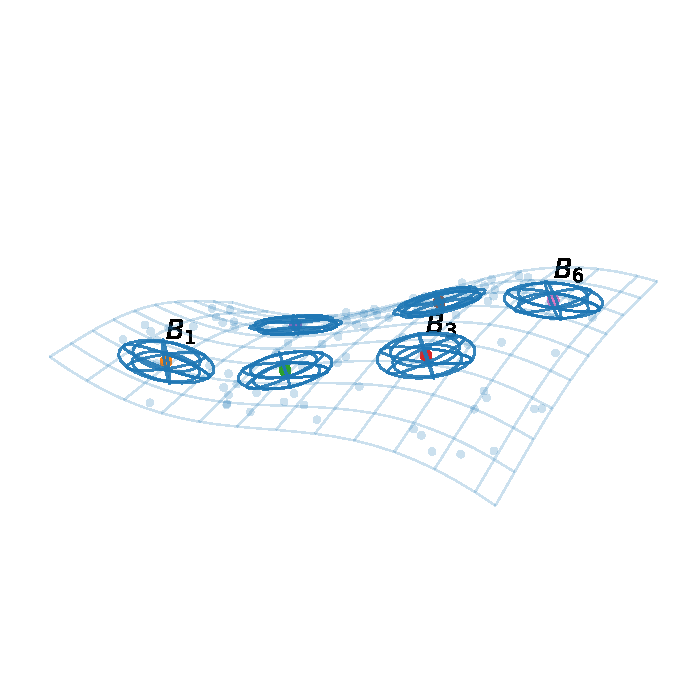
\includegraphics[width=10.1cm,height=3.5cm,keepaspectratio]{manifold3d.pdf}
\par\vspace{0.06cm}
{\large\textbf{Huynh Thanh Dat}}\quad{\normalsize 14 September 2026}
\vspace{0.28cm}
\par{\small Baselines $\;\to\;$ Baseline results $\;\to\;$ NBD $\;\to\;$ Comparison}
\end{center}
\end{frame}

\def\phase{PROBLEM}
\begin{frame}[t]{One-class detection}
\vspace{0.23cm}
\begin{columns}[T,onlytextwidth]
\column{.40\textwidth}
\head{Train on normal data}
\[
\mathcal D_N=\{x_i\}_{i=1}^{n}.
\]
\vspace{0.15cm}
\head{Score new observations}
\[
s(x):\mathcal X\to\RR.
\]
A larger score means more anomalous.
\vspace{0.30cm}
\band{Training and calibration: normal only.\\[0.1cm]Test: normal + anomaly.}
\column{.56\textwidth}
\centering
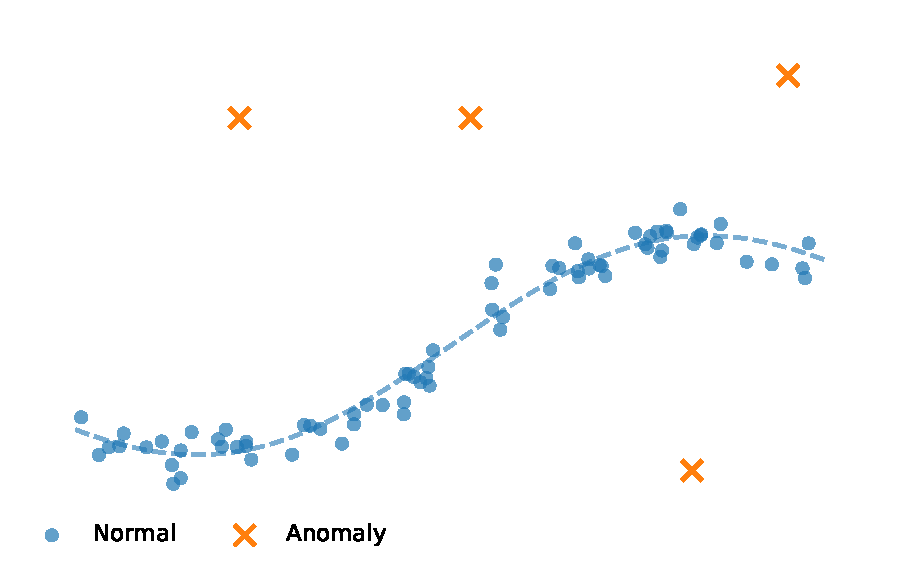
\includegraphics[width=\linewidth,height=4.8cm,keepaspectratio]{problem.pdf}
\src{Schematic: normal support can be curved.}
\end{columns}
\vspace{0.28cm}
\remarktext{Executed MVTec benchmark: $z_p=f_{\rm CNN}(x)_p$; all measured variants share frozen descriptors.}
\end{frame}


\def\phase{ORIGINAL SOURCE}
\begin{frame}[t]{PatchCore: the authors' released feature pipeline}
\small
\textbf{PatchCore} is the paper method. \textbf{PatchScore} below is our nearest-memory baseline.
\par\vspace{.10cm}
\begin{center}
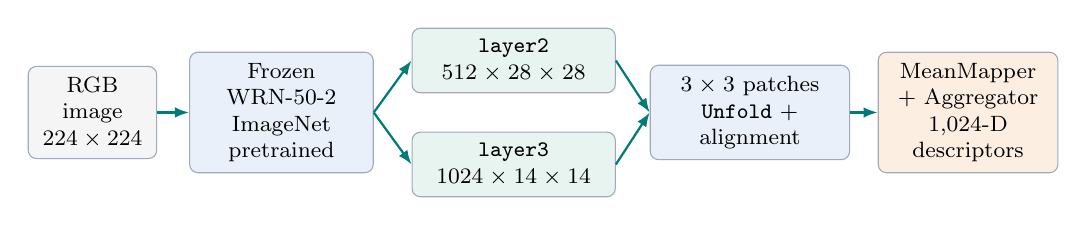
\begin{tikzpicture}[
 b/.style={rounded corners=3pt,draw=navy!40,align=center,inner sep=4pt,font=\footnotesize,minimum height=.82cm},
 a/.style={-{Latex[length=1.8mm]},thick,draw=teal}]
\node[b,fill=softgray,text width=1.35cm] (im) at (0,0) {RGB image\\$224\times224$};
\node[b,fill=softblue,text width=2.05cm] (cnn) at (2.40,0) {Frozen WRN-50-2\\ImageNet pretrained};
\node[b,fill=softgreen,text width=2.30cm] (l2) at (5.35,.66) {\texttt{layer2}\\$512\times28\times28$};
\node[b,fill=softgreen,text width=2.30cm] (l3) at (5.35,-.66) {\texttt{layer3}\\$1024\times14\times14$};
\node[b,fill=softblue,text width=2.25cm,minimum height=1.05cm] (pat) at (8.35,0) {$3\times3$ patches\\\texttt{Unfold} + alignment};
\node[b,fill=softorange,text width=2.0cm,minimum height=1.05cm] (emb) at (11.12,0) {MeanMapper\\+ Aggregator\\1,024-D descriptors};
\draw[a](im)--(cnn);\draw[a](cnn.east)--(l2.west);\draw[a](cnn.east)--(l3.west);
\draw[a](l2.east)--(pat.west);\draw[a](l3.east)--(pat.west);\draw[a](pat)--(emb);
\end{tikzpicture}
\end{center}
\vspace{.02cm}
\begin{columns}[T,onlytextwidth]
\column{.48\textwidth}
\head{Released 224-pixel baseline}
Resize 256; center crop 224.\\
Approximate greedy coreset: \textbf{10\%}.\\
One nearest neighbor; \textbf{max} patch score.
\column{.48\textwidth}
\head{What our measured run changed}
Average-pool + concatenate: \textbf{1,536-D}.\\
128 local-mean centers; top-\textbf{1\% mean}.\\
Same CNN does not imply the same method.
\end{columns}
\vspace{.15cm}
\band{\footnotesize Paper Eq. (7) includes score reweighting; the pinned release uses max NN distance. Keep these variants distinct. Native rerun results are not yet available.}
\vfill
\src{\gitref{https://github.com/amazon-science/patchcore-inspection/tree/fcaa92f124fb1ad74a7acf56726decd4b27cbcad}{GitHub: amazon-science/patchcore-inspection} \;|\;
\gitref{https://github.com/amazon-science/patchcore-inspection/blob/fcaa92f124fb1ad74a7acf56726decd4b27cbcad/sample_training.sh}{run recipe} \;|\;
\gitref{https://github.com/amazon-science/patchcore-inspection/blob/fcaa92f124fb1ad74a7acf56726decd4b27cbcad/src/patchcore/patchcore.py}{feature extraction} \;|\; Roth et al., CVPR 2022.}
\end{frame}

\def\phase{METHODS}
\begin{frame}[t]{PatchScore: shared CNN, normal memory}
\small
\begin{columns}[T,onlytextwidth]
\column{.49\textwidth}
\centering
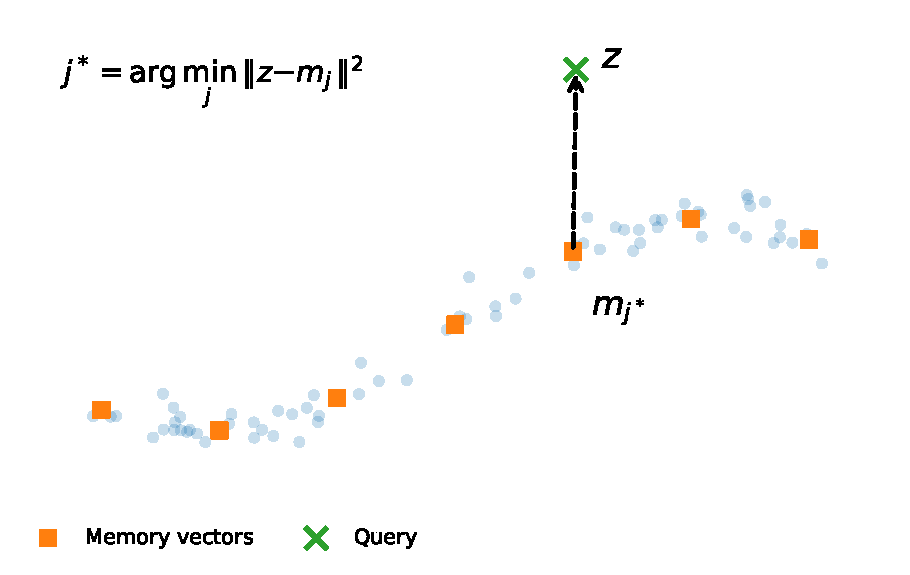
\includegraphics[width=\linewidth,height=2.60cm,keepaspectratio]{patchscore.pdf}
\par\vspace{0.10cm}
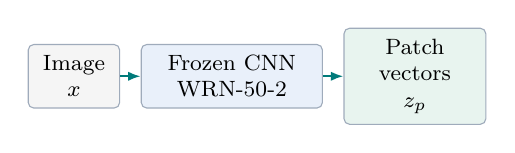
\begin{tikzpicture}[
box/.style={rounded corners=2pt,draw=navy!40,align=center,inner sep=4pt,
minimum height=.80cm,font=\footnotesize},
arr/.style={-{Latex[length=1.6mm]},thick,draw=teal}]
\node[box,fill=softgray,text width=.88cm] (x) {Image\\$x$};
\node[box,fill=softblue,text width=2.02cm,right=.26cm of x] (f) {Frozen CNN\\WRN-50-2};
\node[box,fill=softgreen,text width=1.52cm,right=.26cm of f] (z) {Patch vectors\\$z_p$};
\draw[arr](x)--(f);\draw[arr](f)--(z);
\end{tikzpicture}
\par\vspace{.15cm}
\[
s_{\rm PS}(z)=\min_{m_j\in\mathcal M}\norm{z-m_j}_2^2.
\]
\column{.47\textwidth}
\head{Backbone used in this benchmark}
\textbf{Wide ResNet-50-2}, frozen/eval.\\
ImageNet-1K V1; \texttt{layer2 + layer3}.\\[.10cm]
Resize 256; center crop 224.\\
After $3\times3$ \texttt{Unfold}, \texttt{layer3} has a $14\times14$ patch grid.\\
It is bilinearly interpolated to $28\times28$ with \texttt{align\_corners=False}, then matched location-by-location with \texttt{layer2}.\\
$28\times28$ patches; 1,536-D each. No global PCA.
\vspace{.18cm}
\head{Memory for the baseline comparison}
\textbf{128 normal centers.} Select farthest-first anchors from fit patches; take the mean of each anchor's 128-neighbor set.\\[.12cm]
Score a query by its nearest center. A larger-memory control is compared later.
\end{columns}
\vspace{.06cm}
\band{\small All methods use the \textbf{mean of the top 1\% patch scores} for each image.}
\vfill
\resultsrc{Measured adaptation; not full PatchCore. \gitref{https://github.com/amazon-science/patchcore-inspection/tree/fcaa92f124fb1ad74a7acf56726decd4b27cbcad}{Original GitHub}.}
\end{frame}


\def\phase{METHODS}
\begin{frame}[t]{SVDD family: kernel first, then deep}
\vspace{0.05cm}
\begin{columns}[T,onlytextwidth]
\column{.48\textwidth}
\head{1. Kernel SVDD}
\centering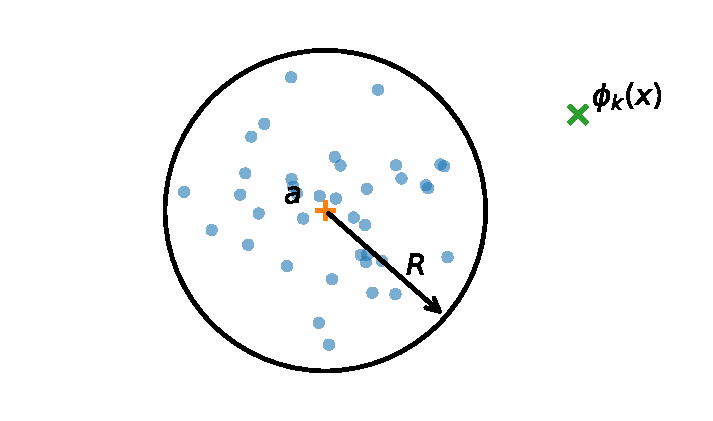
\includegraphics[width=.92\linewidth,height=2.30cm,keepaspectratio]{svdd.pdf}\par
\raggedright\small
\[
\min_{a,R,\xi\ge0} R^2+C\sum_i\xi_i,
\]
\[
\text{s.t. }\norm{\phi_k(z_i)-a}^2\le R^2+\xi_i.
\]
\[
s_{\rm SVDD}(z)=\norm{\phi_k(z)-a}^2-R^2.
\]
\remarktext{Dual QP on 2,048 normal coreset patches.\\$\nu=0.1$; bandwidth from median pair distance.}
\column{.48\textwidth}
\head{2. Deep SVDD}
\centering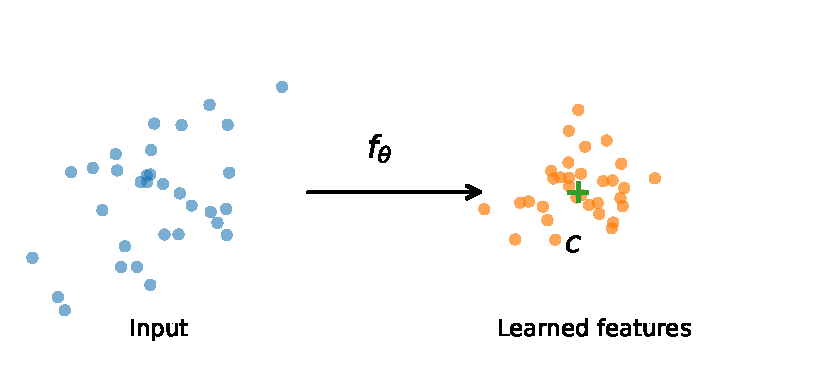
\includegraphics[width=.99\linewidth,height=2.30cm,keepaspectratio]{deep_svdd.pdf}\par
\raggedright\small
\[
\min_\theta\frac1n\sum_i\norm{g_\theta(z_i)-c}^2
+\frac\lambda2\norm\theta^2.
\]
\[
s_{\rm DSVDD}(z)=\norm{g_\theta(z)-c}^2.
\]
\vspace{0.04cm}
\remarktext{Bias-free $1536\to64\to16$ head; fixed $c\ne0$.\\50 AE + 100 SVDD epochs; all fit patches.}
\end{columns}
\vspace{0.2cm}
\src{Measured adaptations. \gitref{https://github.com/DMJTax/dd_tools/tree/efaaf04efae1f8be78906836a5d31547b48be7af}{SVDD: author toolbox}\;|\;\gitref{https://github.com/lukasruff/Deep-SVDD/tree/e20f18c8d0ad9dc01cad09fdf311bd861351a9ad}{Deep SVDD: original GitHub}\;|\;\gitref{https://github.com/dathuynh1108/OCC/tree/91223d63adc3289786bbdeff16d5feeb59aeb3d7/nbdbench}{Our executed code}.}
\end{frame}

\def\phase{METHODS}
\begin{frame}[t]{Deep SVDD: collapse and safeguards}
\small
\remarktext{Shared-CNN setup: $z$ is a frozen descriptor; only $g_\theta$ is trained.}
\vspace{0.10cm}
\begin{columns}[T,onlytextwidth]
\column{.47\textwidth}
\head{Collapse $\ne$ compactness}
Normal compactness is intended. A constant mapping loses all input information.
\begin{alertblock}{Trivial mapping}
\[
 g_\theta(z)\equiv c\quad\Longrightarrow\quad s(z)=0.
\]
\small Normal and anomalous queries get the same score.
\end{alertblock}
\vspace{0.08cm}
A bias provides an easy constant-map solution:
\[
 g_\theta(z)=Wh(z)+b,\quad W=0,\ b=c.
\]
\remarktext{Only the data term is necessarily zero.}
\column{.49\textwidth}
\head{Controls in the current code}
\textbf{No bias.} Both trainable head layers use
\texttt{bias=False}.
\par\vspace{0.11cm}
\textbf{Fixed nonzero center.} Compute $c$ once from normal outputs; do not optimize it.
\par\vspace{0.11cm}
\textbf{ReLU.} Avoid bounded activations with nonzero saturation.
\par\vspace{0.11cm}
\textbf{AE pretraining.} Reconstruct normal features, then discard the decoder before SVDD.
\end{columns}
\vspace{0.09cm}
\band{\footnotesize AE gives an initialization, not a guarantee against collapse.
The code logs final output variance as a diagnostic.}
\vfill
\src{Ruff et al., ICML 2018, Sec. 3.3. \gitref{https://github.com/lukasruff/Deep-SVDD/tree/e20f18c8d0ad9dc01cad09fdf311bd861351a9ad}{Original GitHub}\;|\;\gitref{https://github.com/lukasruff/Deep-SVDD-PyTorch/tree/1901612d595e23675fb75c4ebb563dd0ffebc21e}{Authors\textquotesingle\ PyTorch port}. Controls above refer to our trained head.}
\end{frame}

\def\phase{METHODS}
\begin{frame}[t]{DROCC-head: negatives in CNN feature space}
\small
\begin{block}{Normal label: 1 \hspace{0.4cm} Generated label: 0}
\[
\min_\theta\frac1n\sum_i\left[\ell(g_\theta(z_i),1)
+\mu\max_{r\le\norm{h}_2\le\gamma r}\ell(g_\theta(z_i+h),0)\right]
+\frac\lambda2\norm\theta^2.
\]
\end{block}
\vspace{0.05cm}
\begin{columns}[T,onlytextwidth]
\column{.43\textwidth}
\centering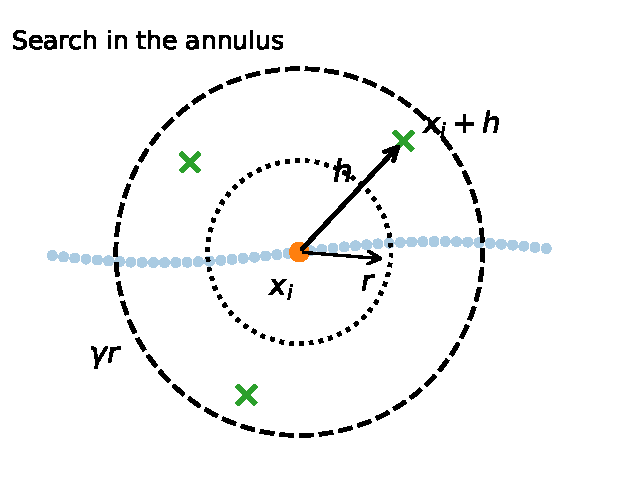
\includegraphics[width=\linewidth,height=3.40cm,keepaspectratio]{drocc.pdf}
\column{.53\textwidth}
\head{Training}
Warm up on normal data.\\[0.08cm]
Ascend in $h$; project back to the annulus.\\[0.08cm]
Update $\theta$ to separate the two labels.
\vspace{0.19cm}
\head{Settings used}
$1536\to64\to1$ MLP; 100 epochs (10 warm-up).\\
50 ascent steps; $\gamma=2$, $\mu=1$.\\
$r=0.5\times$ median normal 5-NN distance.\\
Ascent step $0.05r$; score $s(z)=-g_\theta(z)$.
\end{columns}
\resultsrc{Feature-space adaptation. Batch 8,192; all fit patches. \gitref{https://github.com/microsoft/EdgeML/tree/81025fce8ba28707eabe72e11bf3987a8d745608/examples/pytorch/DROCC}{Original GitHub: EdgeML / DROCC}.}
\end{frame}

\def\phase{SHARED SETUP}
\begin{frame}[t]{MVTec AD: shared evaluation setup}
\small
\vspace{.10cm}
\begin{center}
\renewcommand{\arraystretch}{1.30}
\begin{tabular}{lrrr}
\toprule
&\textbf{Train normal}&\textbf{Test normal}&\textbf{Test anomaly}\\
\midrule
All 15 categories&3,629&467&1,258\\
\bottomrule
\end{tabular}
\end{center}
\vspace{.12cm}
\begin{center}
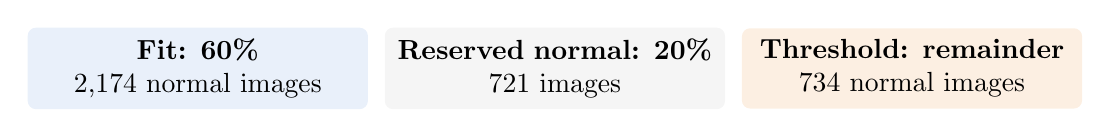
\begin{tikzpicture}[box/.style={rounded corners=3pt,minimum height=1.02cm,text width=4.04cm,align=center,inner sep=4pt}]
\node[box,fill=softblue] (fit) {\textbf{Fit: 60\%}\\2,174 normal images};
\node[box,fill=softgray,right=.20cm of fit] (reserved) {\textbf{Reserved normal: 20\%}\\721 images};
\node[box,fill=softorange,right=.20cm of reserved] (thr) {\textbf{Threshold: remainder}\\734 normal images};
\end{tikzpicture}
\end{center}
\remarktext{Per-seed totals across categories. Split by image, before extracting patches.}
\vspace{.08cm}
\textbf{Reserved images are unused by these four baselines.} Fit on the left subset; set image thresholds on the right subset.
\par\vspace{.18cm}
Same frozen CNN descriptors and splits; seeds \textbf{0, 1, 2}. All test images retained.\\[.08cm]
Models and thresholds are fixed before testing.
\vspace{.13cm}
\band{\small Metrics: image AUROC / AP and FPR / TPR. Image score: mean of the top 1\% patches.}
\vfill
\resultsrc{\texttt{results/lean-nbd-5070-20260915/REPORT.md}, \texttt{configs/lean\_ad\_bd.json}. Shared-feature comparison; not the original paper benchmarks.}
\end{frame}

\def\phase{BASELINE DIAGNOSTICS}
\begin{frame}[t]{Training diagnostics: Deep SVDD and DROCC}
\small
\vspace{.12cm}
\begin{columns}[T,onlytextwidth]
\column{.48\textwidth}
\head{Deep SVDD-head}
Image AUROC: \textbf{81.15 $\pm$ 0.18\%}.
\begin{block}{Output variance ratio}
\[
\frac{\text{final normal output variance}}{\text{initial normal output variance}}
\]
\small Median: \textbf{0.0008381}.\\[.08cm]
Range: $0.0001495$--$0.0181573$ over 45 runs.
\end{block}
\remarktext{Strong contraction. This alone does not establish a constant mapping or an implementation error.}
\column{.48\textwidth}
\head{DROCC-head}
Image AUROC: \textbf{57.24 $\pm$ 3.52\%}.
\begin{block}{Final training loss}
\small Median: \textbf{1.3862944} over 45 runs.\\[.18cm]
Measured test TPR: \textbf{14.07\%}.
\end{block}
\remarktext{Weak detection in this shared-feature adaptation. This is not the original DROCC paper's benchmark result.}
\end{columns}
\vspace{.20cm}
\band{\small Every fit patch was used in every epoch; batch size 8,192.\\[.08cm]
Terminal checkpoints were used regardless of their test performance.}
\vfill
\resultsrc{Fresh 45-run diagnostics and checkpoints in \texttt{results/lean-nbd-5070-20260915/}.}
\end{frame}

\def\phase{NBD MODEL}
\begin{frame}[t]{NBD: local bubbles, one shared graph}
\vspace{0.13cm}
\begin{columns}[T,onlytextwidth]
\column{.65\textwidth}
\centering
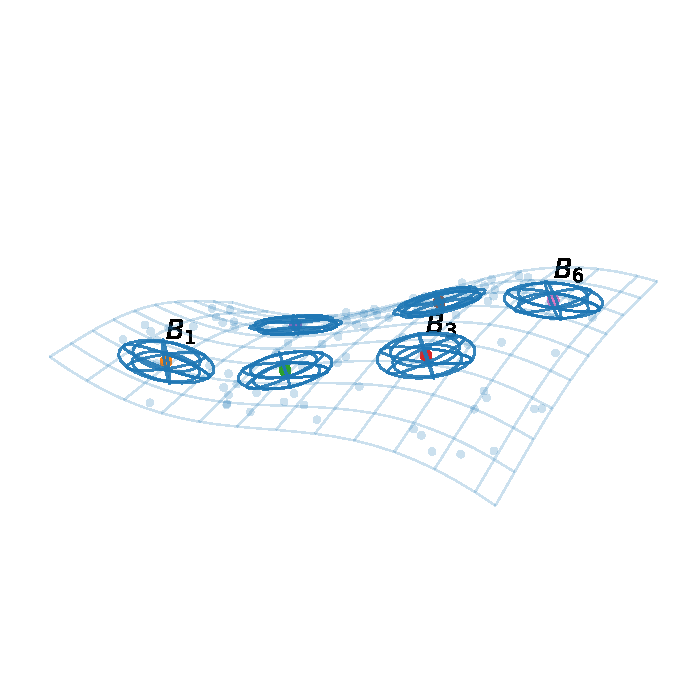
\includegraphics[width=\linewidth,height=4.2cm,keepaspectratio]{manifold3d.pdf}
\src{Schematic: local ellipsoids around a curved surface.}
\column{.31\textwidth}
\head{Each bubble stores}
A center, tangent variation, and normal thickness.
\vspace{0.34cm}
\head{The graph connects them}
Diffusion compares the regions each bubble can reach.
\end{columns}
\vspace{0.28cm}
\band{\centering Normal features $\to$ bubbles $\to$ shared graph $\to$ diffusion distance $\to$ query score}
\remarktext{Hypothesis tested: a normal query has local support and attaches to a coherent region of the graph.}
\end{frame}

\def\phase{NBD MODEL}
\begin{frame}[t]{A local normality bubble}
\small
\[
B_j=(c_j,U_j,\Lambda_j,\sigma_{\perp,j}^2),\qquad
U_j^\top U_j=I_{d_j},\qquad\Pi_j=U_jU_j^\top.
\]
\begin{columns}[T,onlytextwidth]
\column{.57\textwidth}
\head{Local model}
\[
z=c_j+U_ja+\varepsilon_{\perp,j},\qquad a\perp\!\!\!\perp\varepsilon_{\perp,j},
\]
\[
a\sim\mathcal N(0,\Lambda_j),\qquad
\varepsilon_{\perp,j}\sim\mathcal N\!\left(0,\sigma_{\perp,j}^2(I-\Pi_j)\right).
\]
\[
\boxed{\Sigma_j=U_j\Lambda_jU_j^\top+\sigma_{\perp,j}^2(I-\Pi_j).}
\]
\column{.39\textwidth}
\centering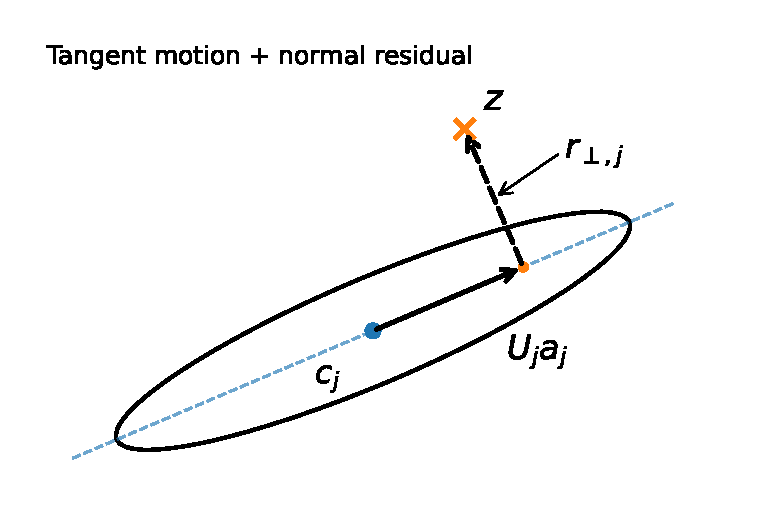
\includegraphics[width=\linewidth,height=2.90cm,keepaspectratio]{bubble_detail.pdf}
\end{columns}
\vspace{0.10cm}
\head{Fit by local PCA}
Neighborhood mean $\to c_j$; top $d_j$ eigenpairs $\to U_j,\Lambda_j$.
\[
\sigma_{\perp,j}^2=\frac1{D-d_j}\sum_{k=d_j+1}^{D}\widehat\lambda_{jk}.
\]
\remarktext{Executed: 128 bubbles; 128 neighbors; $d_j=16$. The same-center control uses the fitted neighborhood means $c_j$.}
\end{frame}

\def\phase{NBD MODEL}
\begin{frame}[t]{Scoring a query}
\small
\[
a_j(z)=U_j^\top(z-c_j),\qquad
r_{\perp,j}(z)=(I-\Pi_j)(z-c_j).
\]
\begin{block}{Local energy}
\[
E_j(z)=
\underbrace{\frac{a_j^\top(\Lambda_j+\epsilon I)^{-1}a_j}{d_j}}_{\text{tangent rarity}}
+\beta\underbrace{\frac{\norm{r_{\perp,j}}_2^2}{(D-d_j)(\sigma_{\perp,j}^2+\epsilon)}}_{\text{off-manifold residual}}.
\]
\end{block}
\vspace{0.02cm}
\begin{columns}[T,onlytextwidth]
\column{.48\textwidth}
\head{Absolute fit}
\[
S_B(z)=\min_{j\in\Cand(z)}E_j(z),
\]
\[
S_A(z)=-T_b\log\!\left[\frac1K\sum_{j\in\Cand(z)}e^{-E_j(z)/T_b}\right].
\]
\column{.48\textwidth}
\head{Attachment to the graph}
\[
b_j(z)=\frac{e^{-E_j(z)/T_b}}{\sum_{k\in\Cand(z)}e^{-E_k(z)/T_b}}.
\]
\remarktext{$K=|\Cand(z)|$ candidates; $b_j=0$ outside.\\$\sum_jb_j(z)=1$.}
\end{columns}
\src{Executed: $K=8$, $T_b=1$, $\beta=1$, $\epsilon=10^{-6}$. This dimension-normalized energy is not Gaussian NLL.}
\end{frame}

\def\phase{NBD MODEL}
\begin{frame}[t]{Comparing two bubbles}
\small
\vspace{0.08cm}
\begin{columns}[T,onlytextwidth]
\column{.322\textwidth}
\head{Center displacement}
\centering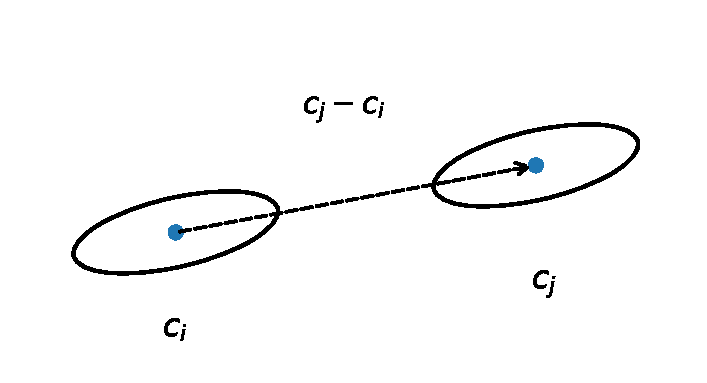
\includegraphics[width=\linewidth,height=1.68cm,keepaspectratio]{pair_centers.pdf}\par\raggedright
\remarktext{Earlier: Euclidean distance}
\[
r_c^{\rm E}(i,j)=\norm{c_i-c_j}_2^2.
\]
\remarktext{Used here: two-way bubble energy}
\[
r_c^{\rm G}(i,j)=\tfrac12\big[E_i(c_j)+E_j(c_i)\big].
\]
\column{.322\textwidth}
\head{Frame geometry inside $D$}
\centering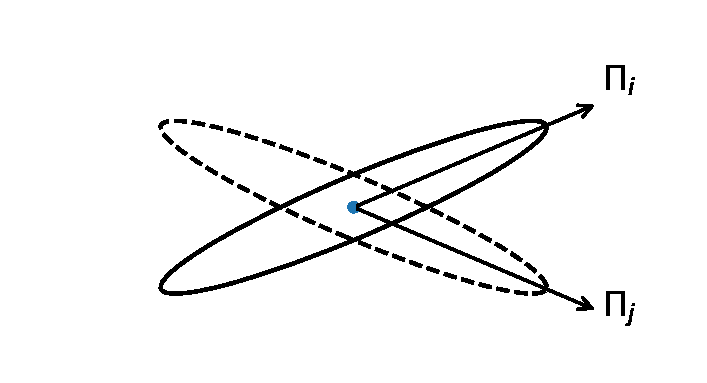
\includegraphics[width=\linewidth,height=1.68cm,keepaspectratio]{pair_frames.pdf}\par\raggedright
\[
r_{\rm frame}(i,j)=\norm{\Pi_i-\Pi_j}_F^2
\]
\[
=d_i+d_j-2\norm{U_i^\top U_j}_F^2.
\]
\remarktext{Compare tangent subspaces, not basis-vector signs.}
\column{.322\textwidth}
\head{Optional: thickness}
\centering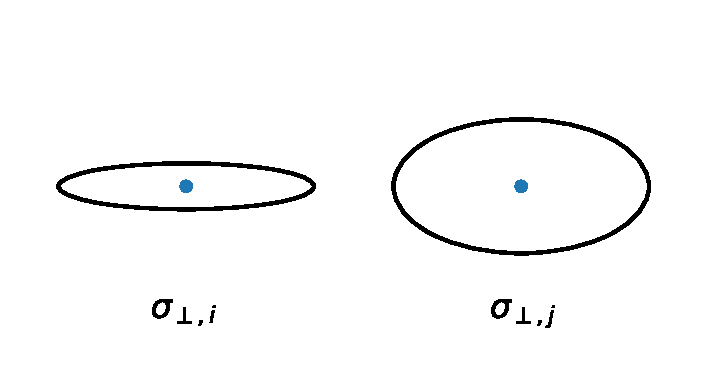
\includegraphics[width=\linewidth,height=1.68cm,keepaspectratio]{pair_thickness.pdf}\par\raggedright
\[
r_\sigma(i,j)=\left[\log\frac{\sigma_{\perp,i}^2+\epsilon}{\sigma_{\perp,j}^2+\epsilon}\right]^2.
\]
\remarktext{Not used in the reported benchmark. Not a full covariance distance.}
\end{columns}
\vspace{0.34cm}
\band{\textbf{Graph inside $D$:} two-way center energy plus frame geometry. Thickness weight is zero.}
\src{The earlier Euclidean distance and the optional thickness term are shown for context, not as tested ablations.}
\end{frame}

\def\phase{NBD MODEL}
\begin{frame}[t]{From bubbles to a graph}
\small
\begin{block}{Edge dissimilarity, before diffusion}
\[
\delta_B(i,j)=\frac{r_c(i,j)}{\tau_c}
+\lambda_{\rm frame}\frac{r_{\rm frame}(i,j)}{\tau_{\rm frame}}.
\]
\end{block}
\begin{columns}[T,onlytextwidth]
\column{.49\textwidth}
\centering\vspace{.20cm}
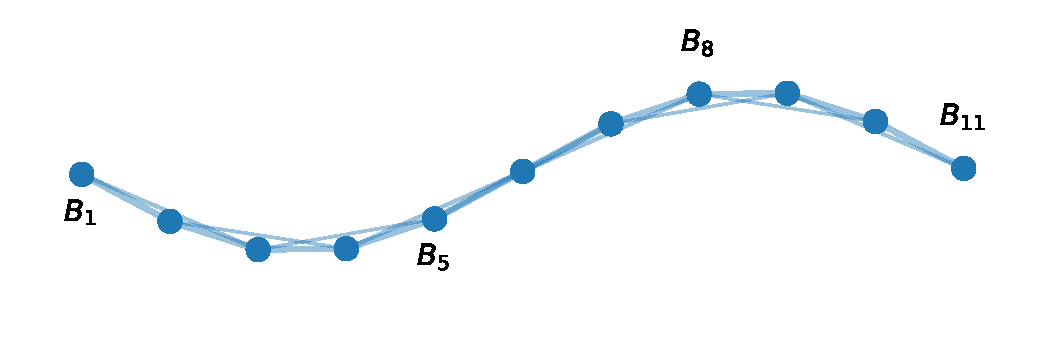
\includegraphics[width=\linewidth,height=2.85cm,keepaspectratio]{bubble_graph.pdf}
\src{Toy graph. Each node is one bubble; thicker edges have larger affinity.}
\column{.47\textwidth}
\head{Affinity and transition}
For symmetric local candidate edges $\mathcal E$,
\[
W_{ij}=\mathbf1_{\{(i,j)\in\mathcal E\}}e^{-\delta_B(i,j)}\quad(i\ne j),
\]
\[
W_{ii}=\eta>0,\qquad s_i=\sum_jW_{ij},
\]
\[
P_{ij}=\frac{W_{ij}}{s_i},\qquad\pi_i=\frac{s_i}{\sum_m s_m}.
\]
\end{columns}
\vspace{0.18cm}
\band{Fit the graph once on normal data. Every query uses the same bubble nodes.}
\src{Executed: 12 graph neighbors; $\lambda_{\rm frame}=1$, $\eta=1$. No thickness penalty. $\delta_B$ need not be a metric.}
\end{frame}

\def\phase{NBD MODEL}
\begin{frame}[t]{Diffusion distance}
\small
Similar $t$-step transition distributions give a smaller diffusion distance:
\[
\boxed{D_t^2(i,j)=\sum_m\frac{\big[(P^t)_{im}-(P^t)_{jm}\big]^2}{\pi_m}.}
\]
\begin{columns}[T,onlytextwidth]
\column{.44\textwidth}
\centering\vspace{0.12cm}
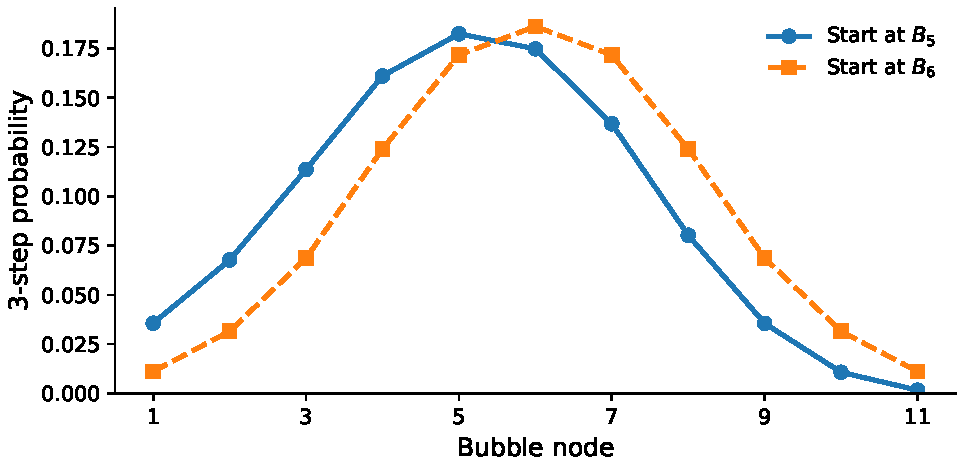
\includegraphics[width=\linewidth,height=2.67cm,keepaspectratio]{diffusion_walks.pdf}
\src{Same toy graph; two neighboring starting nodes, $t=3$.}
\column{.52\textwidth}
\head{Compute with eigenvectors}
\[
P\psi_\ell=\lambda_\ell\psi_\ell,\qquad
\sum_i\pi_i\psi_\ell(i)\psi_k(i)=\delta_{\ell k}.
\]
\[
D_t^2(i,j)=\sum_{\ell=1}^{M-1}\lambda_\ell^{2t}\big[\psi_\ell(i)-\psi_\ell(j)\big]^2.
\]
\[
\Phi_t(B_j)=\big(\lambda_1^t\psi_1(j),\ldots,\lambda_L^t\psi_L(j)\big),
\]
\[
D_{t,L}^2(i,j)=\norm{\Phi_t(B_i)-\Phi_t(B_j)}^2.
\]
\end{columns}
\src{[4] Coifman--Lafon (2006). Executed: all $L=M-1$ nonconstant modes, $\mathcal T=\{1,3,5\}$. The figure is schematic.}
\end{frame}

\def\phase{NBD MODEL}
\begin{frame}[t]{Does the query attach to one region?}
\small
\begin{columns}[T,onlytextwidth]
\column{.48\textwidth}
\centering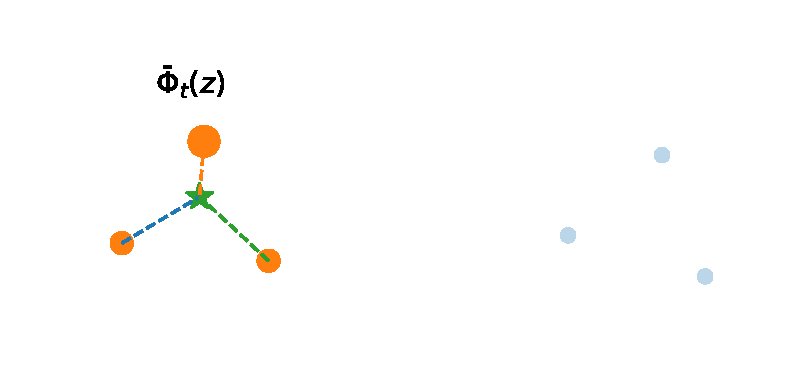
\includegraphics[width=.88\linewidth,height=1.28cm,keepaspectratio]{attachment_near.pdf}
\par\textbf{Nearby bubbles: lower dispersion}
\column{.48\textwidth}
\centering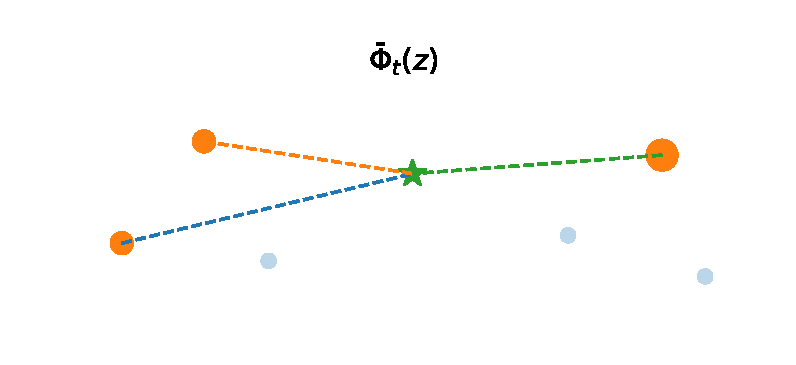
\includegraphics[width=.88\linewidth,height=1.28cm,keepaspectratio]{attachment_far.pdf}
\par\textbf{Distant bubbles: higher dispersion}
\end{columns}
\src{Schematic diffusion coordinates. Circle area: $b_j(z)$. Star: weighted mean.}
\[
\boxed{S_D(z)=\frac1{2|\TT|}\sum_{t\in\TT}\sum_{i,j}b_i(z)b_j(z)D_{t,L}^2(i,j).}
\]
\begin{columns}[T,onlytextwidth]
\column{.50\textwidth}
\head{Equivalent variance at time $t$}
\[
\begin{aligned}
\bar\Phi_t(z)&=\sum_jb_j(z)\Phi_t(B_j),\\[0.2em]
S_{D,t}(z)&=\sum_jb_j(z)\norm{\Phi_t(B_j)-\bar\Phi_t(z)}^2.
\end{aligned}
\]
\column{.46\textwidth}
\head{Why keep a local score}
\remarktext{$D$ measures whether the attached bubbles diffuse together. A query can attach sharply to one bubble and still have $D\approx0$, so $A$ or $B$ remains necessary.}
\end{columns}
\src{A one-bubble outlier can have $S_D\approx0$; $S_B$ and $S_A$ measure absolute local mismatch.}
\end{frame}

\def\phase{NBD MODEL}
\begin{frame}[t]{Lean scoring candidates: one local term plus diffusion}
\small
\setlength{\abovedisplayskip}{3pt}\setlength{\belowdisplayskip}{3pt}
\begin{block}{Two fixed candidates for the fresh RTX 5070 study}
\[
\boxed{S_{A+D}(z)=\widetilde S_A(z)+\widetilde S_D(z),\qquad
S_{B+D}(z)=\widetilde S_B(z)+\widetilde S_D(z).}
\]
\end{block}
\textbf{NBD only:} $\mathcal Z_{\rm cal}$ contains patches from the 721 reserved normal images:
\[
\widetilde S_q(z)=-\log\!\left[
\frac{1+\sum_{u\in\mathcal Z_{\rm cal}}\mathbf1_{\{S_q(u)\ge S_q(z)\}}}{|\mathcal Z_{\rm cal}|+1}
\right],\qquad q\in\{A,B,D\}.
\]
\vspace{0.02cm}
\begin{center}

\begin{tikzpicture}[box/.style={rounded corners=3pt,minimum height=.60cm,text width=3.9cm,align=center,inner sep=4pt},arr/.style={-{Latex[length=2mm]},thick,draw=teal}]
\node[box,fill=softblue] (z) {Patch features $z_p$};
\node[box,fill=softgreen,right=.40cm of z] (a) {Patch scores $A(x)$};
\node[box,fill=softorange,right=.40cm of a] (s) {Image score};
\draw[arr](z)--(a);\draw[arr](a)--(s);
\end{tikzpicture}
\end{center}
\begin{columns}[T,onlytextwidth]
\column{.43\textwidth}
\[
A(x)_p\in\{S_{A+D}(z_p),S_{B+D}(z_p)\}.
\]
\column{.53\textwidth}
\[
S_{\rm image}(x)=\frac1{|\mathcal P_\rho(x)|}\sum_{p\in\mathcal P_\rho(x)}A(x)_p.
\]
\end{columns}
\src{$\mathcal P_\rho$: top 1\% (8 of 784 patches). ECDF scores are not calibrated anomaly probabilities.}
\vspace{0.0cm}
\band{\footnotesize Component scaling uses the reserved subset, not the 734 threshold images.\\[.06cm]
After aggregation, NBD uses the same image-threshold rule as the baselines.}
\end{frame}

\def\phase{LEAN STUDY}
\begin{frame}[t]{Fresh RTX 5070 benchmark: both final scores decrease}
\small
\begin{columns}[T,onlytextwidth]
\column{.47\textwidth}
\head{Locked run}
Frozen Wide ResNet-50-2 ImageNet V1; layer2 and layer3 features concatenate to a 1,536-D descriptor on a $28\times28$ grid.\[.08cm]
Layer3 starts at $14\times14$, then bilinearly upsamples to $28\times28$ with \texttt{align\_corners=False} before concatenation.\[.08cm]
MVTec AD: 15 classes, 3 seeds, 45 completed and checkpoint-replayed runs. Image score is the mean of the top 1\% patches.
\column{.49\textwidth}
\head{Category-macro image AUROC}
\renewcommand{\arraystretch}{1.23}\setlength{\tabcolsep}{3pt}
\begin{tabular}{lrrr}
\toprule
& \textbf{Local} & \textbf{With $D$} & \textbf{$\Delta$ pp}\\
\midrule
$A$ route & $82.47\pm1.75$ & $76.16\pm2.72$ & $-6.31$\\
$B$ route & $82.71\pm1.81$ & $75.64\pm2.64$ & $-7.06$\\
\bottomrule
\end{tabular}\[.14cm]
\remarktext{$D$ already uses frame geometry when graph edges are built. The report has no direct $F$ score or $F$ fusion.}
\end{columns}
\vfill
\band{\small Result: retain both candidates for review, but neither improves its own local component on the category macro.}
\resultsrc{\texttt{results/lean-nbd-5070-20260915/summary.csv}; mean $\pm$ sample SD across three seed macro means.}
\end{frame}

\begin{frame}[t]{Per-class effect of adding diffusion $D$}
\scriptsize
\centering
\renewcommand{\arraystretch}{1.08}\setlength{\tabcolsep}{4pt}
\begin{tabular}{lrr@{\qquad}lrr}
\toprule
\textbf{Class} & \multicolumn{2}{c}{$A{+}D$ vs $A$} & \textbf{Class} & \multicolumn{2}{c}{$B{+}D$ vs $B$}\\
\cmidrule(lr){2-3}\cmidrule(lr){5-6}
& $\Delta$ pp & \textbf{Status} & & $\Delta$ pp & \textbf{Status}\\
\midrule
bottle & -7.67 & reduced & bottle & -8.02 & reduced\\
cable & -12.49 & reduced & cable & -13.77 & reduced\\
capsule & -10.04 & reduced & capsule & -10.53 & reduced\\
carpet & -1.99 & reduced & carpet & -3.09 & reduced\\
grid & -13.92 & reduced & grid & -14.17 & reduced\\
hazelnut & -9.71 & reduced & hazelnut & -9.54 & reduced\\
leather & -5.14 & reduced & leather & -7.78 & reduced\\
metal\_nut & -4.43 & reduced & metal\_nut & -4.77 & reduced\\
pill & +2.37 & improved & pill & +1.45 & improved\\
screw & -4.00 & reduced & screw & -4.09 & reduced\\
tile & +0.47 & improved & tile & +0.63 & improved\\
toothbrush & -3.89 & reduced & toothbrush & -4.26 & reduced\\
transistor & -4.13 & reduced & transistor & -5.76 & reduced\\
wood & -18.33 & reduced & wood & -20.13 & reduced\\
zipper & -1.69 & reduced & zipper & -2.12 & reduced\\
\bottomrule
\end{tabular}
\vfill
\resultsrc{Per-class mean paired AUROC delta over seeds 0, 1, 2. Full SD and all metrics are in \texttt{class\_delta\_report.csv}.}
\end{frame}


\def\phase{REPRODUCTION LINKS}
\begin{frame}[t]{Reproduction sources on GitHub}
\footnotesize
\renewcommand{\arraystretch}{1.35}
\begin{tabularx}{\textwidth}{p{2.1cm}Y >{\RaggedRight\arraybackslash}p{4.35cm}}
\toprule
\textbf{Method} & \textbf{Clickable repository} & \textbf{Role}\\
\midrule
PatchCore & \gitref{https://github.com/amazon-science/patchcore-inspection/tree/fcaa92f124fb1ad74a7acf56726decd4b27cbcad}{amazon-science/patchcore-inspection} & Authors' released code\\
SVDD & \gitref{https://github.com/DMJTax/dd_tools/tree/efaaf04efae1f8be78906836a5d31547b48be7af}{DMJTax/dd\_tools} & Author toolbox; not a 2004 experiment snapshot\\
Deep SVDD & \gitref{https://github.com/lukasruff/Deep-SVDD/tree/e20f18c8d0ad9dc01cad09fdf311bd861351a9ad}{lukasruff/Deep-SVDD} & Original experiment code\\
Deep SVDD & \gitref{https://github.com/lukasruff/Deep-SVDD-PyTorch/tree/1901612d595e23675fb75c4ebb563dd0ffebc21e}{lukasruff/Deep-SVDD-PyTorch} & Later authors' implementation\\
DROCC & \gitref{https://github.com/microsoft/EdgeML/tree/81025fce8ba28707eabe72e11bf3987a8d745608/examples/pytorch/DROCC}{microsoft/EdgeML --- DROCC} & Authors' implementation\\
This benchmark & \gitref{https://github.com/dathuynh1108/OCC/tree/91223d63adc3289786bbdeff16d5feeb59aeb3d7}{dathuynh1108/OCC @ 91223d6} & Our measured adaptation\\
\bottomrule
\end{tabularx}
\vspace{.10cm}
\band{\small Rerun handoff: \texttt{CODEX\_REPRODUCE.md}.\par\vspace{.07cm}\footnotesize
Native paper/release runs first; controlled NBD comparisons separately. Existing MVTec results remain unchanged until new runs complete.}
\vfill
\src{Links pin inspected commits. Original code and our measured adaptations are separate.}
\end{frame}

\def\phase{REFERENCES}
\begin{frame}[t]{References and benchmark files}
\small
\begin{columns}[T,onlytextwidth]
\column{.55\textwidth}
\head{Method sources}
\textbf{[1]} Tax and Duin (2004).\\
\href{https://doi.org/10.1023/B:MACH.0000008084.60811.49}{\emph{Support Vector Data Description.}}\\[.20cm]
\textbf{[2]} Ruff et al. (2018).\\
\href{https://proceedings.mlr.press/v80/ruff18a.html}{\emph{Deep One-Class Classification.}}\\[.20cm]
\textbf{[3]} Goyal et al. (2020).\\
\href{https://proceedings.mlr.press/v119/goyal20c.html}{\emph{DROCC: Deep Robust One-Class Classification.}}\\[.20cm]
\textbf{[4]} Coifman and Lafon (2006).\\
\href{https://doi.org/10.1016/j.acha.2006.04.006}{\emph{Diffusion maps.}}\\[.20cm]
\href{https://github.com/amazon-science/patchcore-inspection}{PatchCore reference implementation}\quad
\href{https://www.mvtec.com/research-teaching/datasets/mvtec-ad}{MVTec AD}
\column{.41\textwidth}
\head{Executed benchmark}
\href{https://github.com/dathuynh1108/OCC/tree/91223d63adc3289786bbdeff16d5feeb59aeb3d7}{\texttt{dathuynh1108/OCC @ 91223d6}}\\[.08cm]
\texttt{results/mvtec-full-v2/}\\
\texttt{REPORT.md}, \texttt{summary.csv}\\
\texttt{category\_summary.csv}\\
\texttt{paired\_deltas.csv}\\
\texttt{SLIDE\_UPDATE\_HANDOFF.md}\\[.16cm]
Locked settings: \texttt{configs/full.json}.\\
Backbone: WRN-50-2, ImageNet-1K V1.
\vspace{.20cm}
\head{This slide package}
\texttt{review.tex}, \texttt{assets/},\\
CSV snapshots and plotting code.\\[.12cm]
Reported audit: 450 metric rows; 51,750 image predictions. Replay: 135 groups; max error 0.0.
\end{columns}
\vfill
\resultsrc{Snapshot: 14 September 2026. Source audit and links only; no new benchmark run.}
\end{frame}
\end{document}
